%% intro.tex

On May 29, 1919 during a total solar eclipse, three scientists, Eddington,
Dyson, and Davidson, tried to find out what effect, if any, is produced by a
gravitational field on the path of a light ray traversing
it~\cite{Eddington1920}.  During a thoroughly prepared expedition, they measured
the deflection of positions of stars in the well-known Hyades constellation
caused by the mass of the Sun as predicted by the theory of gravity, general
relativity.  This was the first observation of gravitational lensing, as well as
the first predicted and validated effect of general
relativity~\cite{Einstein1911}.

Effectively, gravitational lensing is entirely analogous to optical lenses. In
fact, to produce the distorted light signatures like they are observed in
gravitational lens systems, one only needs a stem and the base from a wine glass
and move it in front of a light source.
\href{https://phdenzel.github.io/zurich-lens/}{phdenzel.github.io/zurich-lens/}
provides an interactive toy example of such a situation.  In optics, the lens
comprises a glass sheet of variable thickness.  It deflects light by an amount
proportional to the local depth.  The physical process which causes the change
of direction when a ray traverses a glass lens, is called refraction.  It
describes the delay, i.e. decrease in speed of light, due to the change of media
and therefore a change in direction.  While the result of lensing is the same
for both optical and gravitational lenses, the latter causes the delay and
deflection due to the change of the felt gravitational potential as light moves
through it.  The rather rare occurrence of a perfect alignment of a background
source, a quasar for instance, and a massive foreground lens in which the imaged
source is distorted in a way such that it can be observed multiple times or even
as a ring wrapping around the lens, is called \textit{strong} gravitational
lensing.  \figref{mock-lens} demonstrates such a case with a mock lens.
%
\begin{figure}[h]%
    \centering%
    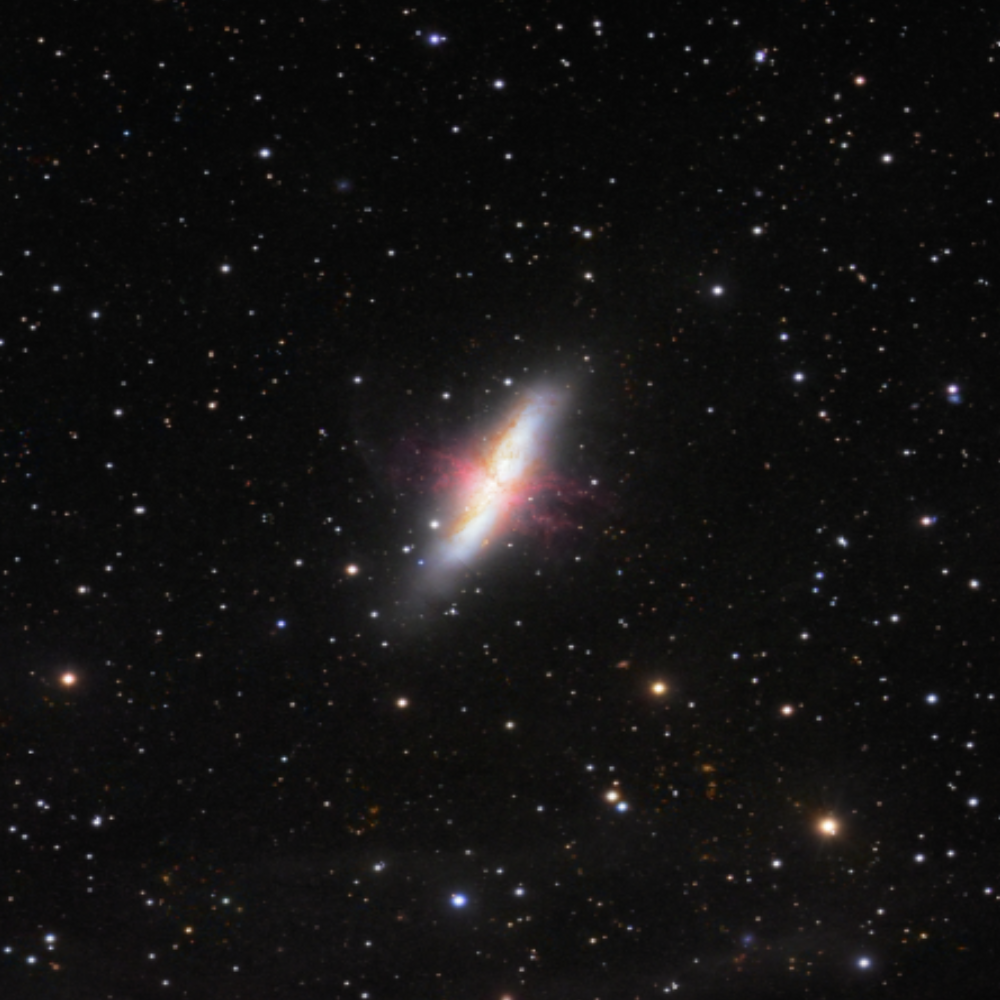
\includegraphics[width=0.49\textwidth]{m82-original}\,%
    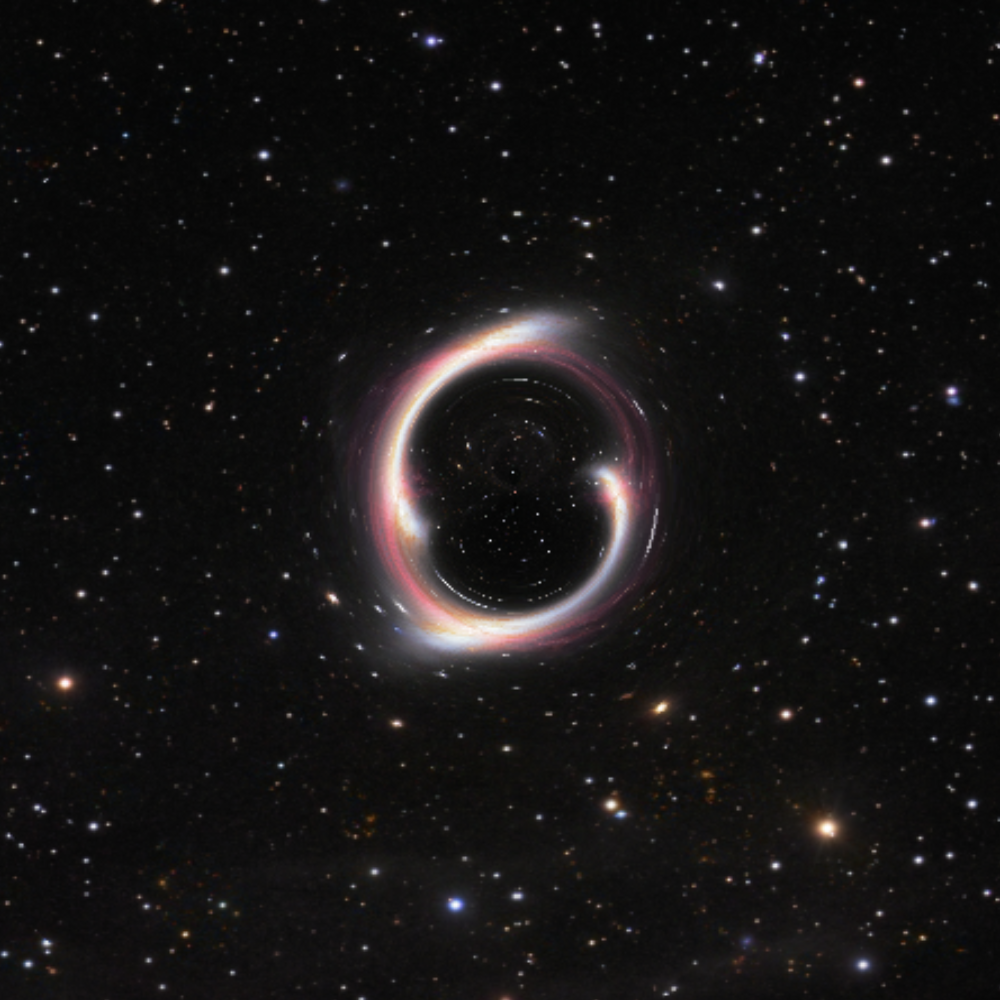
\includegraphics[width=0.49\textwidth]{m82-lensmock}
    \caption[Mock lens image of M82]{Mock lens observation: The left image shows
      the "Cigar Galaxy" M82 cutout from
      \href{https://apod.nasa.gov/apod/ap200515.html}{APOD 2020 May 15}. The
      right image demonstrates what it could look like, if a small black hole
      for instance with 3 times the mass of the Sun would replace the Moon
      (\textcolor{red}{TODO: check calculation again, angular size of 10
      arcmin}).  The right image was generated using my lens mock code:
      \Code{lensing.js}
      (\href{https://phdenzel.github.io/lensing.js/}%
            {phdenzel.github.io/lensing.js/}).\\
      \textit{Image Credit \& Copyright: Dietmar Hager, Torsten
        Grossmann}}%
    \figlbl{mock-lens}%
\end{figure}%
%

More specifically, the deflection in gravitational lensing is of the order of
$4M/R$, where $M$ is the mass of the lens and $R$ its size.  Strong
gravitational lensing occurs when the apparent size $R/D$ of the aligned lens at
a distance $D$ is comparable to that deflection \sidecite{MagicEnv}.  In fact,
although the underlying physical process is all the same, gravitational lensing
is categorised into three types based on the observational techniques and mass
or size regimes: and \textit{micro}, \textit{strong}, and \textit{weak} lensing.
%
\begin{equation}\eqlbl{lensing_types}%
  \begin{aligned}
    \text{micro} \hspace{1cm}&\frac{4M}{R} \gg \frac{R}{D}\\
    \text{strong} \hspace{1cm}&\frac{4M}{R} \gtrsim \frac{R}{D}\\
    \text{weak} \hspace{1cm}&\frac{4M}{R} < \frac{R}{D}
  \end{aligned}
\end{equation}%
%
Microlensing is in many cases due to small, compact, and massive objects such as
stars, or even exoplanets around stars.  While it technically also projects a
source in multiple images, their angular separation is typically of the order of
microarcseconds --- hence the name --- and therefore impossible to resolve with
even the most modern telescopes. Nevertheless, in microlensing the changes in
the source alignments express as changes in apparent brightness, which is
detectable over an observation period of $\sim100$ days.  Weak lensing on the
other hand, happens when the gravitational field of the lens is not strong
enough to create multiple images, and the observable effect is a distortion
which is only detectable in a statistical sense.

Most gravitational lenses lie at cosmological distances, and only very massive,
large, and mass-concentrated objects can in this case lead to strong lensing
features.  Galaxies are vast cosmic islands of stars, gas, dust, and mainly
non-luminous matter held together by gravity.  This puts them in ideal mass and
size range to act as such strong-lensing systems.  Based on most recent
observations, it is estimated that there are more than 2 trillion galaxies in
the Universe \sidecite{Conselice16}, however so far less than a thousand
gravitational lenses have been found across various data sets.  This makes them
quite the rare beasts in comparison\dots\ at least for now.  Future space and
ground-based telescope missions however, such as the \textit{Square Kilometer
Array} (SKA), the \textit{Vera Rubin Observatory} (formerly known as
\textit{Large Synoptic Survey Telescope}, or LSST), the \textit{James Webb Space
Telescope} (JWST), and \textit{Euclid} are expected to find several orders of
magnitudes more.  This is very promising for science, because, due to their very
special circumstances, lensing galaxies and their configurations can be modelled
and give otherwise unobtainable insights into galaxy structure. The task of lens
models is to describe particular shapes of the lensing galaxy's mass
distribution which produces deflections of one or more background sources which
agree with the observed lensed images.  The fact that gravity and thus lensing
is indiscriminate of the kinds of matter which cause the deflections, makes it
all the more interesting.  In this regard, gravitational lenses are often seen
as 'proof'\sidenote{Not the only proof, as explained in following sections.} for
invisible and non-luminous matter, commonly called \textit{dark matter}, without
which the observed deflections due to galaxies cannot be explained by general
relativity.

Finding connections between these matter components, how they assembled, and how
they dynamically interact within galaxies is still subject of ongoing research.
Solving galaxy formation and evolution is a crucial part in understanding the
evolution of the Universe as a whole and the physical laws driving it.  During
the last two decades, large-scale hydrodynamical simulations have yielded great
successes and managed to produce galaxy models which agree with astronomical
observations incredibly well.  In contrast, lens models still struggle to
conform with physical properties and are hard to interpret.  Some describe lens
reconstruction techniques as 'black art' \sidecite{SaasFee}, perhaps because
they produce models which are, if at all, only barely motivated by physical
processes which are believed to be key in the dynamics of galaxies. Another
reason might be the confusion seeded by very opposing opinions\sidenote{Excerpt
from \citeay{SaasFee}: "I will argue that the parametric models are all that is
needed to model lenses and that they provide a better basis for understanding
the results than non-parametric models (but the reader should be warned that if
Prasenjit Saha was writing this you would probably get a different opinion)."}
of how these lens models should be constructed.  Nevertheless, while there are
advocates for certain (and not other) approaches, they all agree that these lens
systems are, scientifically speaking, highly valuable and promise to uncover
mysteries surrounding galaxy evolution, the nature of dark matter, galaxy
substructures, and the expansion of the Universe.

The main theme of this thesis is to explore old and new ways of connecting the
three cornerstones of lensing research, \textit{lensing galaxies} from
observations, \textit{lens models} which try to reproduce observations, and
\textit{simulations} of galaxies.  The following chapters detail projects with
that aim, each designated by a project name: \Code{DELAYS}~(\chref{delays}),
\Code{FOSSIL}~(\chref{fossil}), \Code{ADLER}~(\chref{adler}), and
\Code{MATCH}~(\chref{match}).

%
\begin{figure}[h]%
    \centering%
    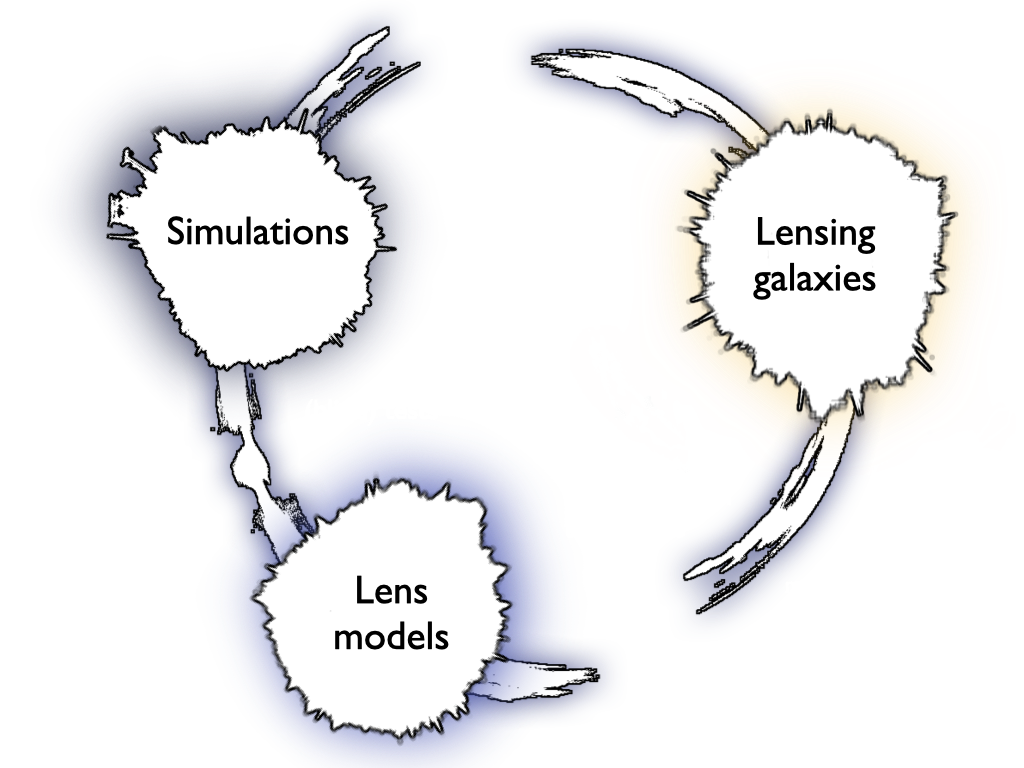
\includegraphics[width=0.99\textwidth]{scheme}%
    \caption[Conceptual graph]{Conceptual graph: the outline of this fictional
        lensing system perfectly construes the current state of lensing
        research.  Simulations of galaxies have been shown to be physically
        realistic and have successfully been inferred by lens models in (blind)
        tests.  However, lens models still struggle to uniquely describe lensing
        galaxies in observations and a direct link from simulations to lensing
        galaxies has so far never even been explored before.  The projects in
        the subsequent chapters thematise these subjects and their connections.
        }%
    \figlbl{concept}%
\end{figure}%
%

Attempts to describe lensing galaxies with models of lens systems have been made
since the very first discovery by~\sideciteay{Walsh1979} in 1979.  In
\chref{delays} and \chref*{fossil}, new techniques were developed to optimise
lens recovery --- still rather traditionally --- with time delay measurements or
stellar population synthesis models respectively.  Even with more physical
information on the lensing galaxies, the models were difficult to properly
constrain and revealed certain issues and limitations.  The subsequent project
in \chref{adler} reports on a blind test which further explores these problems
with mock lenses from large-scale hydrodynamical simulations.  Particularly hard
to solve is the issue of degeneracies, the fact that a lens configuration can be
caused by many, differently shaped lenses, which is a long-known, inherent
limitation to lens models.  It also proposes analysis techniques which can be
employed in this case to isolate these problems.  Finally, \chref{match} gives
proof-of-concept for an entirely new form of lens modelling, a 'matching'
technique, which provides a direct link from simulations to lensing galaxies in
observations.

The following sections introduce the subsequent chapters and cover some basics
and related topics in the schematic of \figref{concept}.  They elaborate on a
few key aspects in cosmology (\secref{exp_universe}), some basic lensing theory
(\secref{lensing}), and theoretical and observational background related to
galactic dynamics, in particular focusing on topics relevant to galaxies in
lensing systems (\secref{galaxies}).  Finally, the subsequent chapters are put
into context and shortly summarized.

%\clearpage
\section{The expanding Universe}\seclbl{exp_universe}
%% exp_universe.tex

% Discovery of the expanding universe
Like most fundamental theories in physics which helped in the present-time
understanding of our Universe and the interactions within, general relativity
was formulated in the early 20th century.  While the word was spreading of
Einstein's construct of the supposedly quasi-static Universe which involved a
'cosmic constant' to keep it so, Vesto Melvin Slipher and Edwin Hubble performed
the key measurements which provided the connection between theory and
observations.  By 1923, Slipher's hard work yielded a compilation of velocity
estimates for 41 galaxies.  Remarkably, most of those galaxies were receding
from us, and thus appeared redshifted\sidenote{The recession velocity of a
galaxy can be measured by the (Doppler) shift of its spectral lines, i.e.
redshift.}.  Half a decade afterwards, Edwin Hubble investigated the relation
between his distance measurements to these galaxies and their radial velocities.
Thereby, he effectively measured an apparently constant velocity gradient in
units of \Hunitsalt.  This constant was later named after him, the
\textit{Hubble constant}~\Ho.  Through this velocity gradient he realised
something, which could arguably be called the birth of modern cosmology: the
concept of an expanding Universe would explain why all galaxies are receding
from us and each other~\sidecite{Kirshner04,
Hubble1929}\marginnote[0.75cm]{While one would expect such a finding to be
highly cited, Hubble's publication interestingly counts only 73 official
citations at the time of writing.}.  The outward motion of galaxies resulting
from the uniform expansion of the Universe is best observable at very high
distances where the local, mutual gravitational interaction between galaxies is
subdominant.  This behaviour is commonly referred to as the \textit{Hubble
flow}.

Hubble's realisation was an impressive leap of thought, even more so, since the
prevalent idea of the Universe at the time was synonymous to today's picture of
our own galaxy, the Milky Way, beyond which the existence of anything else was
uncertain.  Only around 1920, astronomers started considering that what they
called nebulae were in fact extra-galactic 'island universes' that is entirely
other galaxies.  Today, there are 'standard' recipes for recreating and
improving upon Hubble's results\sidenote{He determined the Hubble constant by
the slope of his iconic diagram with roughly $\Ho \approx 500\,\Hunits{}$.} by
gathering distance and velocity or redshift estimates to galaxies and other
astronomical objects which are much further away.  While this might seem like a
simple task, the matter of measuring distances relates to problems with which
cosmology struggles still today.  

The most 'human' method of measuring distances is the \textit{parallax}.  It
essentially utilises the same principles as the human eye.  With two points of
observation, an astronomical, stereoscopic vision is achieved from which the
distance can be estimated.  However, with even the most sophisticated
technologies reaching high angular resolution, parallax has only very little
reach.  Since the main objective in cosmology is to study the Universe's
large-scale structures from birth to the present, this technique is relatively
ineffective as it rarely reaches objects able to probe the Hubble flow.  Still,
it is generally used as calibration for other techniques with longer reach.  An
especially powerful application of the parallax is the measurement of distances
to galaxies containing megamasers, gas clouds with water molecules which
catalyse the emission of coherent microwave radiation.  Distances to these
emission points can be determined to incredible precision with long baseline
interferometers and spectral monitors.  Another strong influence of the parallax
technique is reflected in the distance unit 'parallax second' which is usually
shortened to \textit{parsec} and ubiquitously employed in astronomy and
astrophysics.  It is the distance where 1 astronomical unit (AU; the nominal
distance of Earth to the Sun) spans 1 arcsecond on the sky.  Using \ref{eq:au}
and \ref{eq:arcsectan}, we can write:
%
\begin{equation}%
    1\,\parsec = 1\,\AU \times \tan(1\,\arcsec)^{-1} \approx 10^{8}\,\lightsec
    \eqlbl{parsec}
\end{equation}%
%
Distance measurements sensitive to the expansion of the Universe have to rely on
different strategies.

In an expanding, flat Universe many different measures of distances can be
defined.  For example, it can be very useful to factor out the expansion and
define the so-called \textit{comoving distance}
%
\begin{equation}\eqlbl{d_comov}%
    d_{comov} = \frac{c}{\Ho} \int_0^{z} \frac{d\zeta}{\sqrt{\Omega_m(1+\zeta)^3
    + \Omega_r(1+\zeta)^4 + \Omega_\Lambda}}.
\end{equation}
%
where $z$ is the redshift of the light to which the distance is measured, and
$\Omega_i=\rho_i/\rho_c$ are the relativistic, non-relativistic, and dark energy
components, normalised by the cosmological critical density $\rho_c$.  Every
component contributes at various scales differently to the expansion or
contraction of the Universe, and therefore have to be considered separately when
distances are measured.  In a flat Universe, the cosmological critical density
is its average density $\propto\Ho{}^{2}/G$.  The comoving distance does not change with time,
assuming the observers are moving with the Hubble flow.  Another measure which
is especially often used in the context of lensing, is the
\textit{angular-diameter distance} which is defined as an object's physical size
over the its angular size as viewed from Earth. It can also be written as
%
\begin{equation}\eqlbl{d_comov}%
    d_{ang} = \frac{d_{comov}}{(1+z)}
\end{equation}
%
It is the distance which freezes the Universe at the time when the light which
is used to measure it, is emitted.  This leads to a very peculiar behaviour that
beyond some redshift the angular-diameter distance actually decreases with
increasing redshift.

For a long time, light from very bright sources represented the only way of
measuring distances in astronomy\sidenote{As explained below, gravitational
waves changed the game in more than one way.}.  Just like lighthouses acted as
distance markers and warning signals for reefs and promontories to mariners
since ancient times, bright light sources called \textit{standard candles}
provide the means for the most common method to determine distances for the
purpose of probing the Hubble flow.  For such objects, the intrinsic luminosity
$L$ can be measured or determined theoretically without measuring their
distance.  By observing their apparent light flux $F$ dimmed by traversing the
vastness of space, a \textit{luminosity distance} can be determined
%
\begin{equation}\eqlbl{d_lum}%
    d_{lum} = \sqrt{\frac{L}{4\pi F}}
\end{equation}%
%
which happens to relate with $d_{lum}={(1+z)\,d_{comov}}$ to the comoving
distance.  Cepheids for instance, variable stars for which the intrinsic
luminosity depends on their periodic behaviour of brightness fluctuations, are
long-known standard candles.  Their luminosity-period relation was discovered by
Henrietta Leavitt in 1912 and enabled the first distance measurements reaching
past the edge of the Milky Way to the Andromeda Galaxy (M31).  The brightest
standard candles known to astronomers however are Type-1a Supernovae (SNeIa).
They are a special variant of Supernova in which a white dwarf in a binary star
system accretes mass.  Due to this process, the exact energy available at the
time of Supernova and thus its standardizable intrinsic luminosity is given by
the Chandrasekhar mass limit of $1.44\mathrm{M_\odot}$.  

Yet withal there is no single method which is applicable to all ranges of
distances.  Thus, a common procedure in the measurement of the Hubble constant
is the \textit{cosmic distance ladder}, in which one distance measurement
iteratively provides calibration for the next, with the end of the rung being
the farthest reaching SNeIa.  Methods based on the distance-redshift relation
are often called 'late' measurements.

Opposed to these are the 'early' measurements, which are based on completely
different physical processes.  Instead of a distance measurement, the 'early'
measurements determine the Hubble constant and other cosmological constants,
with angular modes of temperature on the Cosmic Microwave Background (CMB).  For
instance, the monopole temperature of the CMB evolves with $\dot{T}_{\text{CMB}}
= -\Ho{}T_{\text{CMB}}(t)$.  The current temperature of the CMB is known to be
around $T(0) = 2.725\;\mathrm{K}$. So, with a Hubble constant of the order of
$70\;\Hunitsalt{}$, this yields a change in temperature of roughly
$-0.2\;\mathrm{nK/yr}$ and could be measured with accurate detectors over a long
period of time.  The common method however to infer \Ho{} is based on the
multipole-temperature fluctuations of the CMB.  The particular structure at
angular sizes in the CMB arises due to baryonic acoustic oscillations (BAO)
which are an imprint of pressure waves in the primordial baryon-photon plasma.
Therefore, the amplitudes of the BAO peaks depend on the baryon-density
component of the Universe through which the Hubble constant can be indirectly
determined.  Such methods obtain estimates which are independent of the cosmic
distance ladder employed by 'late'-Universe measurements.

The separation between 'early' and 'late' measurements of the Hubble constant
has been emphasised in the last decade, because of a discrepancy in the results
they yielded.  While measurements of late-Universe probes indicate a Hubble
constant of around $\Ho = 74.0 \pm 1.4\;\Hunitsalt$~\sidecite[][latest results
obtained by the SH0ES (Supernovae \Ho\ for the Equation of State) project which
measures the Hubble constant using Supernovae]{Riess19}, 'early'-Universe
measurements generally yield a lower value of $\Ho = 67.4 \pm
0.5\;\Hunitsalt$~\sidecite[][most recent inference of the cosmological
parameters from the Planck collaboration]{Planck18b}.  In the comparison of the
values and uncertainties of such determinations, it becomes apparent that there
is a discrepancy at a $4.5\sigma-5.5\sigma$-level\sidenote{depending on the
exact measurements being compared} between these two opposing sides.  This means
that there is roughly a 1 in 20'000'000 chance of both measurements being
different on accident, which indicates a problem with either one or both
methods.  The seemingly only way to resolve this so-called \textit{Hubble
tension}, without completely changing the concordance model of cosmology, is to
find some so-far unknown systematic errors in the measurements which would
account for the discrepancies.  As it currently stands however, the Hubble
tension appears to force the rejection of the most successful cosmological
concordance model, the $\Lambda$ cold-dark matter model ($\Lambda$CDM). 

For this reason, it is crucial to have as many independent methods of obtaining
estimates for the Hubble constant as possible, each with sufficient precision to
resolve the tension.  In the past couple of years, gravitational lenses were
believed to provide a third perspective on the issue and possibly resolve the
discrepancies surrounding the value of \Ho{}.  While other methods are based on
standardizable luminosity measurements or the angular power spectrum of the CMB,
gravitational lenses induce differences in travel times of light rays, so-called
time delays, which can be measured in the lensed images of quasars and other
time-variable sources over a period of the order of years.  These time delays
set the scale of the lensing system and are proportional to the inverse of the
Hubble constant, the Hubble time.  Through these time delays, the recovery of
the lensing-mass distribution therefore allows an independent measurement of the
Hubble constant from a completely different physical process.  

\chref{delays} presents a critical study of such a measurement.  With an
analysis on 8 time-delay lenses, I determined the Hubble constant with a value
of \sidenote{\protect\textcolor{red}{TODO}: I was told that one should use 'I'
in the intro... is this really what is usually done?}
%
\begin{equation*}%
    \Ho = 71.8^{+3.8}_{-3.3}\;\Hunitsalt
\end{equation*}%
%
The value is compatible with both the early and late measurements, with a
tension of less than $1.5\sigma$.  With a precision of 4.9\%, the measurement is
unfortunately not able to contribute to the resolution of the Hubble tension.
In fact, the investigation revealed that, if a 1\% level is at all obtainable,
it would require a joint-analysis of many more time-delay measurements of
quadruply imaging lens systems (quads).  It was not the only determination of
the Hubble constant through lensing observations recently; the H0LiCOW
collaboration \sidecite{Wong19} reported on a Hubble constant of
$73.3^{+1.7}_{-1.8}\;\Hunitsalt$ from 6 time-delay lenses a year before, and the
STRIDES collaboration \sidecite{Shajib20} determined a value of
$74.2^{+2.7}_{-3.0}\;\Hunitsalt$ from a single lens.  However, while these
results were reported with higher confidence, this study explores many different
lens models and thus accounts for lensing degeneracies by construction.
Although degeneracies are often neglected in lensing studies, it is known for a
long time that a family of lens-mass distributions is able reproduce the same
observables, but still yield different values for the Hubble constant.
Therefore, studies with the aim of inferring the Hubble constant need to solve
for (ideally) all possible solutions of mass distributions in order to retrieve
a complete model.  The study produced 8000 lens-mass distributions with 1000
values for the Hubble constant.  Most interestingly, the values appeared to be
asymmetrically distributed, which might indicate that the errors on \Ho{} could
be non-Gaussian.  These results were not entirely unexpected since the
investigation was actually a continuation of ideas gathered during a
participation in a scientific blind study \sidecite{TDLMC2} in which 50
simulated time-delay lenses were analysed by several research groups.  It
discovered that current lens recovery methods are accurate to only about 6\%,
even with acclaimed precision over nearly 1\%.  In comparison with the study
presented in \chref{delays}, it became apparent that the lens simulations
considerably differed from real observations and that the uncertainties in the
inference of \Ho{} from mock lenses were higher.  Besides the obvious numerical
deviations, the radial distribution of lens images of the simulated lens set was
relatively narrow which provided only little constraints on the slope of the
density profile and consequently on \Ho.  This could mean that there exists a
limit to the accuracy on \Ho{} achievable with time-delay galaxy lenses, which
ultimately might preclude them to infer \Ho{} on a level required to resolve the
Hubble tension.  Nonetheless, gravitational lenses are excellent cosmological
probes. Especially cluster lenses do not exhibit this limitation and might still
recover the Hubble constant with sufficient precision to contribute to the
resolution of the Hubble tension.

Even so, it is unlikely for a single method to resolve the Hubble tension alone.
However, another promising approach to determine distances has emerged.  Light
signals weaken with the square of their distance as described by \eqref{d_lum}.
This means a signal will be 4 times less bright at twice the distance, which is
generally the case for long-range physical laws, be it the gravitational force,
electro-magnetic force, or most kinds of radiation.  Of course, for a constant
progress out into the cosmos, the demand on technologies is twice as high and
pushes them to their limits.  Recently however, the detection of gravitational
waves changed the game.  When two massive, compact objects such as black holes
orbit each other and start to inspiral, some amount of energy is emitted in form
of gravitational waves\sidenote{a highly non-classical effect!}.  A major
advantage over their electro-magnetic counterpart is that the signal strength of
gravitational waves decreases with distance linearly.  The benefits of this
become immediately apparent: if one would manage to build a detector which is
100 times as sensitive, it could measure distances 100 times as far into the
Universe, rather than 10 times as far with a light detector which was 100 times
as sensitive.  The reason for the linear dependence on distance lies in the
method how the signal is generated and measured.  The easiest way of generating
electro-magnetic waves is to move charges back and forth which creates dipole
radiation, commonly known as light.  Due to the conservation of momentum, this
is not possible for gravitational waves which instead consist of quadrupole
radiation.  These kinds of radiations are fundamentally different when it comes
to their detection.  While light simply gets absorbed in the detector and
changes the energy level of the detected signal, gravitational waves induce
stretching and compression in the detector, called strain which is proportional
to the amplitude of the wave.  While the energy of gravitational waves still
falls with the square of the distance, their amplitude decrease with the
distance linearly, which is ultimately the reason of the farther reach of
distance measurements based on gravitational waves.  In the future, this method
of measuring distances will be crucial in resolving the discrepancies in the
measurements of the Hubble constant.

%\clearpage
\section{Lens models}\seclbl{lensing}
%% lensing.tex

General introduction to lens theory and lens modelling.

%%%%%%%%%%%%%%%%%%%%%%%%%%%%%%%%%%%%%%%%%%%%%%%%%%%%%%%%%%%%%%%%%%%%%%%%%%%%%%%%	
\par\noindent\rule{\textwidth}{0.8pt}

The distance to the lens and the source $D_\mathrm{S}$ are always much larger
than the line-of-sight extent of the lens itself. This is what allows the
so-called \textit{thin-lens} approximation which allows the definition of a
projected surface-density distribution
%
\begin{equation}\eqlbl{match:thinlens}
  \kappa(\bm\theta) = \frac{4\pi GD_\mathrm{LS}D_\mathrm{L}}{c^2D_\mathrm{S}}
    \int \rho(\bm\theta, z)\,\mathrm{d}z
\end{equation}
%
from a mass-volume density $\rho$, where $D_\mathrm{LS}$ is the angular-diameter
distance from the lens to the source, $\bm\theta$ the lens plane and $z$ the
line-of-sight coordinate.

% Lensing galaxy models
In this context, it is very useful to think of an arbitrary surface-density
distribution in terms of multipoles:
%
\begin{equation}\eqlbl{match:multipoles}%
  \kappa(\bm\theta) = \langle\kappa_0(\theta)\rangle_{\phi} 
  + \sum^{\infty}_{m=1} \langle\kappa_{m}(\theta)\rangle_{\phi} e^{im\phi}
\end{equation}%
%
where the individual components $\langle\kappa_{m}(\theta)\rangle_{\phi}$ are
angular averages over the surface density, expressed in polar coordinates.  It
corresponds much to the idea that galaxies consist of a main body of matter and
many smaller substructures orbiting around it.  The monopole $\kappa_0$, dipole
$\kappa_1$ and quadrupole $\kappa_2$ are usually considered the most important
components.  While the monopole only leads to radial deflections, the
higher-order multipoles also include angular terms which are composed of two
parts containing the interior and exterior poles.  The angular structure in the
lens is mainly determined by three sources: (i) the luminous lens galaxy
including its stars, gas, and dust, (ii) the dark matter in the halo of the
galaxy, and (iii) the perturbations from nearby objects or objects along the
line of sight.  The most common angular term included by lens models is the
external shear which describes the exterior poles of the quadrupole.

% Lensing degeneracies
In fact, \sideciteay{Young1981} reported the first lens model which already
involved all components up to the quadrupole expressed in terms of an elliptical
mass distribution using a small set of parameters.  Already then, they
identified essentially every important lensing-related issue, and in particular
realized that there are many different mass distributions which can lead to
identical lensing configurations \sidecite{Young1981b}; these degeneracies
represent an inherent limitation to lens reconstructions \sidecite{Saha2000}.
They create many misconceptions about lens models even amongst experts, as often
times a single family of models is not able to fully describe lensing
observables \sidecite{Gomer19, Denzel20, Kochanek20, TDCOSMO4}.  To reduce or
even break degeneracies, modern lens reconstruction techniques try to constrain
their models with additional data besides the image positions such as relative
fluxes of the images, arc-like extended images, stellar photometry to describe
the dynamics of the lensing galaxies, or time delays between the images
\sidecite{Barnabe07, Ferreras07, Auger10, Bruderer15, Leier11, Leier16,
Nightingale19, Denzel20b, Shajib20, Wong19}.
%\clearpage
\section{Galaxies}\seclbl{galaxies}
%% galaxies.tex

The current scientific consensus within the cosmological paradigm is that all
matter in the Universe was created roughly a Hubble time ($\Ho^{-1} =
13.7\;\Gyrs$) ago during a singularity known as the Big Bang.  Afterwards, a
rapidly expanding and cooling phase began, and all matter was almost uniform in
distribution.  Over the course of these several billion years, spontaneous
fluctuations on top of this uniform distribution grew, slightly denser regions
of matter became gravitationally bound to each other.  Eventually, they formed
primordial galaxies of hydrogen gas enveloped by a large dark matter halo.  In
these proto-galaxies, cold and over-dense molecular clouds gravitationally
collapsed to form the first stars.  These stars were rather massive and burnt
through their hydrogen fuel quickly.  Such stars generally end in violent
supernovae through which they reintroduce heavier elements\sidenote{commonly
termed \textit{metals} in astrophysics whose aggregates form \textit{dust}} back
into their gas environment, the \textit{interstellar medium} (ISM).  The
interplay of these components form a dynamical, self-regulatory, but chaotic
system and settle into a morphological state of the galaxy.  The study of these
dynamical processes and their correlations therefore can uncover crucial clues
to the formation history and structure of galaxies. 

The endeavour of measuring the dynamics of galaxies was and still is
complicated, even more so within the Milky Way.  Earth is revolving around our
Sun, and the Solar System is orbiting around the Galactic centre, which means
relative motions have to be carefully examined.  From some locations on Earth, a
dense strip of starlight is visible across the night sky which is indicative of
the Galaxy's disk structure.

\begin{figure}[h]
    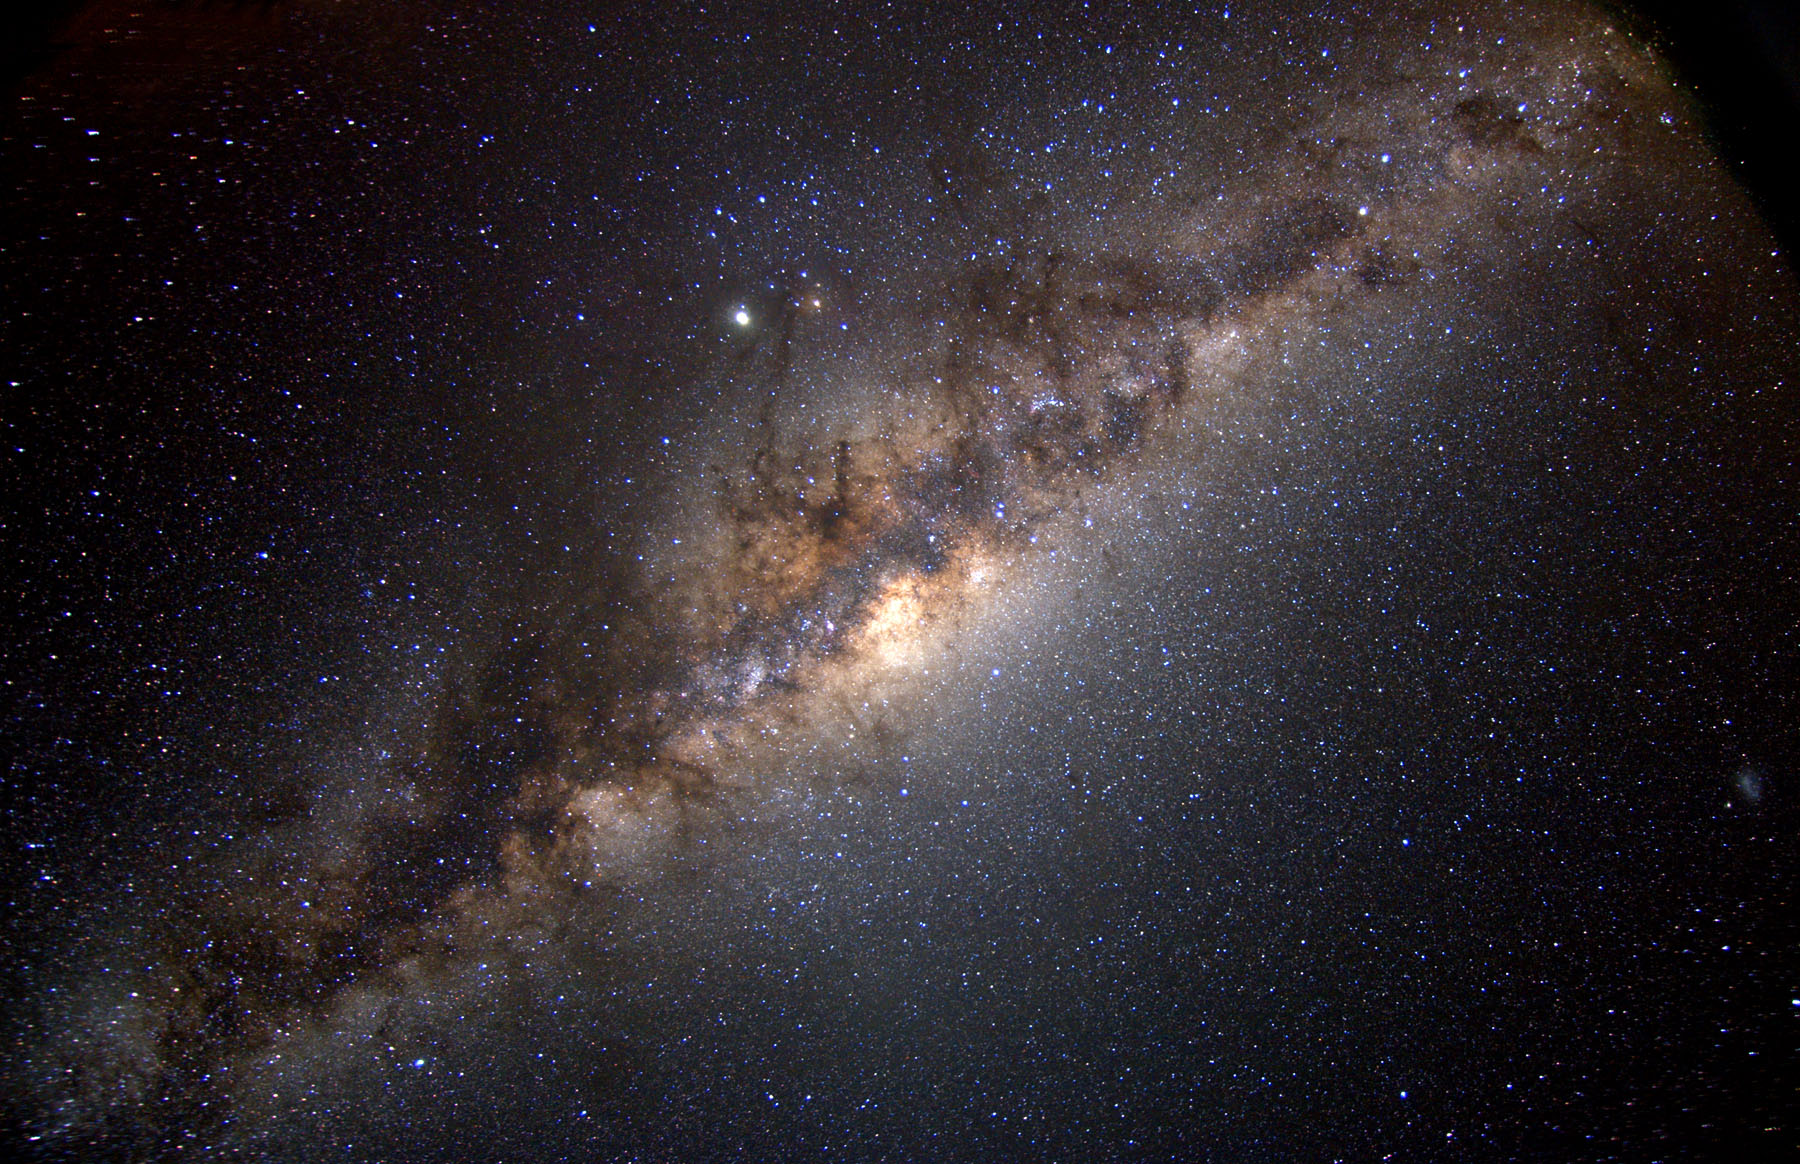
\includegraphics{apod080104}
    \caption[The Milky Way: APOD 2008 January
    4]{\href{https://apod.nasa.gov/apod/ap080104.html}{APOD 2008 January 4}: The
    Milky Way at 5000 meters.\\
    View on our own galaxy from within (recorded in the Chilean Andes).  The
    band of the dense collection of stars from the disk and the Galactic centre
    is partially covered by the typical extinction features due to dust
    clouds.  It indicates that the Milky Way possesses a stellar disk.\\
    \textit{Credit \& Copyright: Serge Brunier}}
    \figlbl{milkyway}
\end{figure}

From far away it is quite easy to recognise the typical morphology of other
galaxies through direct observations\sidenote{provided the telescope has enough
angular resolution}.  Measuring their rotational properties already becomes
increasingly difficult, but deducing the shape and rotation patterns of the
Milky Way from within is an undertaking of its own.

A seemingly random and dense distribution of stars as it appears in galaxies
should in principle collapse towards its potential well.  Despite the expansion
of the Universe, this would eventually lead to the collapse of entire galaxies
into their centres.  Like in many other astrophysical scenarios, pressure
gradients can take a stabilising role, balance gravity, and thereby prevent
complete collapse.  These balancing pressures depend on different physical
processes and generally define limiting scales.  For some galaxies, e.g.
ellipticals, the stars' random motions are the dominant drivers towards
stability, for spiral galaxies it is the rotation about their disk's centre.  In
contrast to orbiting systems such as the Sun and Earth, where most of the mass
is located near the guiding centre of the orbits, the Milky Way's mass
distribution is more complex and extended with different elements such as
various forms of hydrogen gas, dust, stars, and stellar remnants.  In general,
the study of galactic rotation through stars can yield insights not only into
the galaxy's morphology, but also into its formation history and mass
composition.  

Weighing galaxies is not an easy task either, partially because most of their
components are invisible, dark matter being the most elusive amongst them.
However, much like tree branches move in the wind, orbits of stars still feel
the gravitational pull from the mass inside them, independent of the nature of
the matter.  Stars in a more massive galaxy will move with higher orbital speeds
than in lower-mass galaxies; more formally, the mass $M$ inside the (circular)
orbit of radius $r$ is $M(<r) \propto V^{2}r$, where $V$ is the orbital speed of
the star.  Accordingly, by measuring the velocities of stars at a particular
distance from the centre, a mass estimate for the galaxy can be calculated,
which is a simple application of Newton's first law combined with Kepler's law.
It is equivalent to assuming the galaxy is in hydrostatic equilibrium formulated
by the virial theorem 
\begin{equation}
    \begin{aligned}
        &V^{2} = \frac{M(<r)}{r}\\
        &2E = -U,
    \end{aligned}
\end{equation}
where $E$ and $U$ are the kinetic and potential energy respectively
\sidecite{BinneyTremaine08, Zwicky1933}.  When the individual orbits of stars
cannot be resolved in {e.g.} spiral galaxies, other 'tracers' can be used such
as atomic hydrogen gas measured through 21-cm line radiation in the radio
spectrum \sidecite{vandeHulst1951, Muller1951, vandeHulst1954}, or as
perturbations in the optical wavelengths.  For ellipticals, the velocity
dispersion $\sigma$ measured by the spread of spectral absorption lines is the
observable which analogously measures their mass as $M(<r) \propto \sigma^{2}r$
\sidecite{Schechter80, Davies83}.  The observables measured are, in most cases,
treated as dynamical equilibria, or temporal averages and therefore yield (by
implicitly assuming the ergodic theorem) 1-dimensional (1D) models such as the
rotation curve $V(r)$ \sidecite{Bosma17, Ablimit20, Cautun20}.  It characterises
the orbital velocity as a function of distance from the galactic centre. By
measuring how $V(r)$ behaves with increasing radius, we can draw conclusions
about the Milky Way's size, total mass, and the distribution thereof.  For
instance, a solid-body rotation $V \propto r$ would mean that the enclosed mass
ideally increases with $r^{2}$, Keplerian orbits go as $V \propto r^{-\half}$,
whereas $V \propto \text{const.}$ is a result of the enclosed mass increasing as
$r$.  This makes it a powerful tool to investigate the mass distribution of
galaxies.

However, on rare occasions, some galaxies can function as strong gravitational
lenses, and reveal even more details about their internal structure.  These rare
phenomena occur when a source aligns with a massive galaxy acting as a lens and
is multiply imaged or appears as an Einstein ring.  This depends on the
gravitational potential of the galaxy which in turn is related to its entire
mass and the distribution thereof.  As a consequence, the separation of the
images to the lens is determined by the mass inside (see the strong lensing case
of \eqref{lensing_types}), which is typically of the order of $1\,\arcsec$ for
galaxies at cosmological distances.  Moreover, lenses are rarely perfectly
aligned and circular in the real world, but have angular structure, which
produces distorted configurations of source images.  This is what allows us to
go beyond 1D models and infer a lens model in form of a 2D mass distribution
(more details on this are discussed in \secref{lensing}).  Hence, gravitational
lenses provide a unique opportunity to study distant galaxies and their
structure on scales which are difficult to infer with other methods.
Unfortunately, this type of analysis is limited to lensing systems which are
relatively rare, as previously mentioned.  To get an idea of just how rare such
lensing events are, we will next try to estimate the number of lensed sources
based on the Milky Way's kinematics.

The Milky Way's rotation curve can be probed through its stars directly. To that
end, the relevant observables are the radial velocity $v_{z}$, the tangential
velocity $v_{t}$, distance from Earth $d$, and the longitude on the sky $l$.
Measurements of these quantities can be combined to the so-called \textit{Oort's
constants}
%
\begin{equation}\eqlbl{obs_oortsC}%
    \begin{aligned}%
        &A = \frac{v_{z}}{d\sin{2l}} \\
        &B = \frac{v_{t}}{d} - A\cos{2l}.
    \end{aligned}%
\end{equation}%
%
A caveat is the assumption that the stars, including the Sun, are on circular
orbits, which is only approximately true.  Moreover, it assumes the Milky Way
has a monotonically decreasing, symmetric potential.  Again, this is not
entirely true as spiral arms can introduce over-densities which manifest as
asymmetries and locally break monotonic behaviour in the potential.  Still,
within their limits the Oort's constants are very useful, because they can be
rewritten as
%
\begin{equation}\eqlbl{oortsC}
    \begin{aligned}%
        &A = -\frac{1}{2} \left[\frac{\derivd V}{\derivd r}
                                - \frac{V_{0}}{R_{0}}\right] \\
        &B = -\frac{1}{2}\left[\frac{V_{0}}{R_{0}}
                               + \frac{\derivd V}{\derivd r}\right].
    \end{aligned}%
\end{equation}
%
Recent measurements from the Gaia survey determined these constants with
$A=15.3\pm0.4\,\Oortsunitsalt$ and $B=-11.9\pm0.4\,\Oortsunitsalt$
\sidecite{Bovy17}.  These constants express the shear and vorticity of the disk
in the solar neighbourhood.  The shear essentially measures a deviation from
solid-body rotation, the vorticity how the angular momentum varies with small
changes in radius.  Adding both yields the velocity gradient $A+B =
-\frac{\derivd V}{\derivd r}$, which seems to be relatively flat with
$3.4\;\Oortsunitsalt$ as was expected from previous and alternative
investigations.  

From the velocity gradient the mass density for the Milky Way can be estimated
as follows
%
\begin{equation}\eqlbl{MWrho}
    \begin{aligned}
        \rho_{MW} &\quad\sim\quad \frac{(A+B)^2}{2\pi} \\
                  &\quad\sim\quad 10^{-33}\;\sec^{-2}
    \end{aligned}
\end{equation}
%
As a rough estimate, this is of the order of the total mass of the Milky Way
within its size volume $\sim M_{MW} / R_{MW}^3$, as long as the
assumptions of the Oort's constants are valid.  This is obviously not the case
outside the edge of the Galaxy.  However, the size of the Milky Way is not
clearly known.  The issue lies in the ambiguity regarding the definition of the
edge of the Galaxy.  In the literature the '$R_{200}$' is frequently used,
sometimes also called the 'virial' radius within which the mean density equals
200 times the cosmological critical density.  Another less back-of-the-envelope
definition is the 'splashback' radius, a caustic manifested in a drop in density
or radial velocity.  At roughly half the splashback radius an edge can be
defined where virialized material has completed at least two pericentric
passages.  For the Milky Way this radius is at about $R_{MW} \sim
290\;\mathrm{kpc}$ \sidecite{Deason20}, and seems to define an edge where our
assumptions should still hold. 

Generalizing and assuming that the Milky Way is an average galaxy in the
Universe, we can compare the mass density of the Milky Way to the cosmological
matter density
%
\begin{equation}
    \begin{aligned}
        \rho_{m} &=\quad 0.3\times\frac{3\Ho^{2}}{8\pi} \\
                 &\sim\quad 10^{-37}\;\sec^{-2},
    \end{aligned}
\end{equation}
%
which is roughly 30\% of the average energy-density in the Universe.  The ratio
of these two quantities should yield the number of Milky-Way-like galaxies
within the galaxy's volume. Within a cubic volume of $\sim (c/\Ho{})^{3}$ which
corresponds roughly to a tenth of the diameter of the observable Universe and
$10^4$ times farther than the edge of the Milky Way, this number is roughly
%
\begin{equation*}
    10^{12}\times\frac{\rho_m}{\rho_{MW}} \sim 10^{8}.
\end{equation*}
%
Typical strong-lensing galaxies cover roughly an area of $10^{-10}$ square
radians on the sky, which means that within a tenth of the observable Universe
1\% of sources are strongly lensed by galaxies.  Of course, this number is based
on the mass and dimensions of the Milky Way and with it the assumption our
Galaxy be average.  Since the Milky Way is actually more massive than the
average galaxy, the estimate constitutes a lower limit. 

It was further implicitly assumed all galaxies are distributed homogeneously and
isotropically within the considered volume.  These are structural consequences
of what is known as the \textit{cosmological principle}.  It states that on a
sufficiently large scale the properties of the Universe are the same for all
observers, which is equal to say that the same physical laws apply throughout.
Extensive testing of these fundamental postulates to the measurable level seem
to confirm\sidenote{although not conclusively; see \citeay{Migkas20} for a
report of possible deviations from isotropy.} a statistically homogeneous
distribution of galaxies on large scales.  On local scales however, the picture
is much more interesting.  The $\Lambda$CDM model predicts clustering along
filamentary structures within a web-like system of dark matter strings.  Once
formed, galaxies evolved together in larger galactic structures called groups,
clusters and superclusters.  Over time, gravity within these systems forces them
closer and closer, until they eventually collide in a series of mergers. The
outcome of these mergers depends on the mass of the galaxies in the collision.
Smaller 'dwarf' galaxies can be disrupted by larger ones and turned into streams
of stars which orbit the galactic core.  When large galaxies of similar size
come together, their spiral structure is generally lost, and the merged galaxies
become a giant elliptical galaxy.  Through these mergers, a hierarchical
spectrum of various galaxy types forms.

Ultimately, all galaxies within a group or cluster will eventually become
gravitationally bound to each other and merge into a giant elliptical galaxy.
Such almost or fully merged systems are known as 'fossil groups'. They are
always dominated by a single, very luminous and thus massive central galaxy,
around which other galaxies are at least two magnitudes less luminous and
therefore much smaller.  During their comparatively fast merging process, the
intra-group gas medium heats up.  Cooling times in these regions are much higher
than a Hubble time, and thus a large-scale X-ray halo around the original main
galaxy remains.  Fossil groups which have already fully merged, appear today as
massive, completely isolated elliptical galaxies with such group-like X-ray
halos.  As a final product of galaxy merging within a galaxy group, the mass
range of such fossil group galaxies starts at $\sim10^{13}\;\Msol$ and exceeds
the average mass of galaxies by orders of magnitude.  

In recent years, ever more elaborate large-scale hydrodynamical and N-body
simulations have been implemented, which displayed such hierarchical merging
schemes, and produced incredibly realistic galaxies.  Simulations generally use
the field of density fluctuations analogous to the ones observed in the CMB as
initial conditions and progress the entire system in time according to the
cosmological concordance model.  They demonstrate that galaxy formation is
driven by the growth of the underlying large-scale structure and the formation
of dark matter haloes.  Galaxies form through condensation of gas at the centres
of the potential wells of these dark haloes.  The galaxies' subsequent evolution
is usually governed by a plethora of sub-grid models which are adapted to
reproduce properties due to astrophysical effects below the resolution level
such as supernova winds and quasar feedback, in this context often called
\textit{AGN} (active galactic nucleus) feedback.  Based on theoretical
predictions from such simulations, physical properties of galaxies related to
baryons \sidenote{a collective term for all luminous matter in order to
differentiate it from dark matter and dark energy.} should be naturally in tight
correlation with the mass of the dark haloes by which they are hosted.  In
particular, the total mass in stars contained in galaxies reveals interesting
behaviour of how star formation is regulated within, when compared to the mass
of their dark matter halos.

\textit{Halo abundance matching} is a technique which allows such a comparison
and results in an empirical correlation between galaxy and halo properties
\sidecite{Moster12}.  Following an Occam’s razor approach, the technique
directly matches observed galaxy number densities for a given property (such as
luminosity) to theoretical halo number densities obtained through simulations.
The latest Planck survey \sidecite{Planck18b} measured a baryonic-to-total mass
ratio of $\Omega_{b}/\Omega_{m} \sim 0.14$ within the $\Lambda$CDM model.  If
light 'traces' mass this cosmological average should hold for galaxies of all
masses.  Abundance-matched galaxies however indicate that on small scales light
does no longer simply trace mass and predict the star formation of galaxies to
be suppressed at both the low and high ends of the mass spectrum, due to various
astrophysical effects such as tidal stripping\sidenote{depletion of a galaxy's
gas and stellar mass reservoir due to strong tidal forces from neighboring
galaxies}, Supernovae and AGNs.  Generally, having more concentrated baryonic
matter will increase the stellar-to-halo mass fraction while astrophysical
feedback processes which disperses baryonic matter decreases it.  Supernovae
have the tendency to impact galaxies with lower halo masses the strongest by
kinematically removing gas from star-forming regions, whereas AGNs are
especially effective in preventing the formation of stars in higher mass
galaxies through heating and dispersing of the star-forming gas.

In contrast to abundance matching and similar methods which usually rely purely
on theoretical predictions of the halo-mass number density, lensing provides
once again an alternative to compare mass components of galaxies based on
observational estimates.  Since lenses can be used to probe the distribution of
every kind of matter in galaxies, especially the region within the lensed
images, enclosed masses inferred by lens models yield a fair estimate on the
total mass of a galaxy. Through stellar kinematics and colours of the stellar
population in the lensing galaxy, luminous matter can be distinguished from the
dark.  \figref{moster} shows such an analysis for lenses discovered by the
citizen science Space Warps project in comparison with results from abundance
matching by \sideciteay{Moster12}.  Initial modelling of these lenses was done
by a small group of citizen-science volunteers lead by \sideciteay{Kueng18}, and
repeated by me.  For two of these lens models J1434+522 and J2217+015 (annotated
in \figref{moster} with SW05 and SW42, respectively) stellar-mass estimates were
obtained through fitting stellar population synthesis models to the observed
photometry, which yields more precise results compared to the previous estimates
(more details on the stellar-mass estimation are given in \subsecref{fossil} and
\chref{fossil}).

\begin{figure}[h]%
    \centering%
    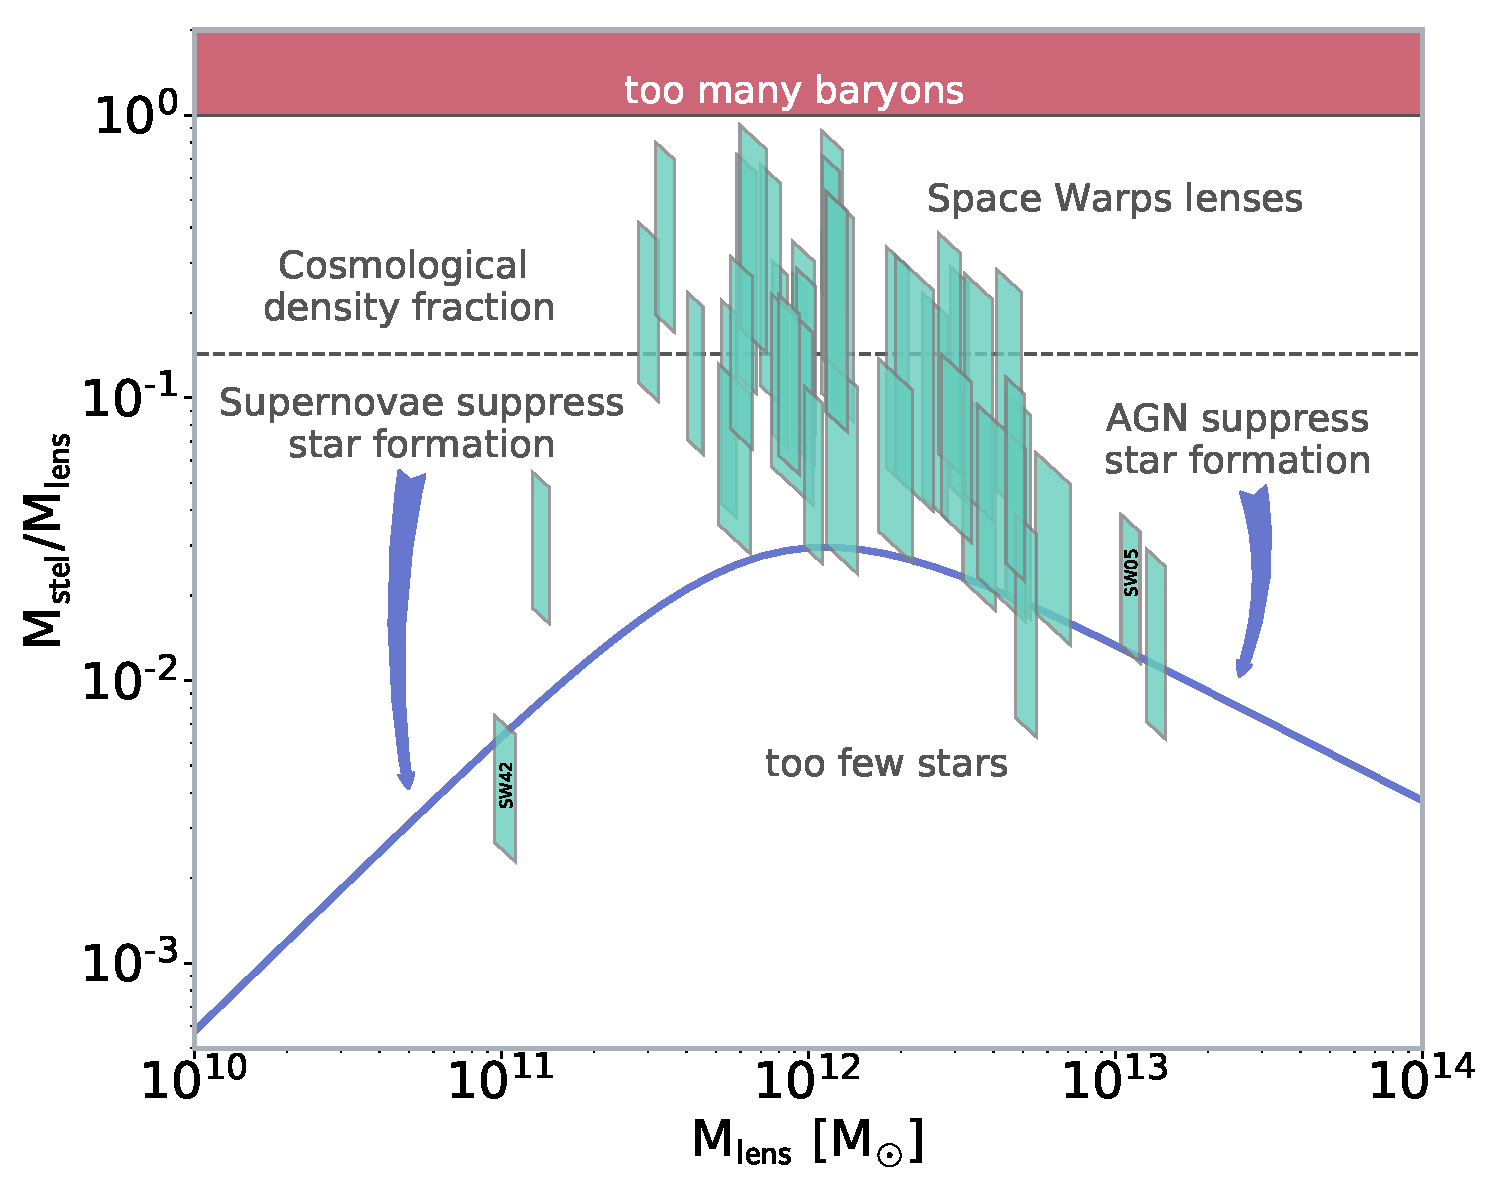
\includegraphics[width=0.99\textwidth]{moster}%
    \caption[Stellar-to-lens mass ratios of lensing galaxies]{Stellar-to-lens
        mass ratios of lensing galaxies (turquoise) from the
        Canada-France-Hawaii Telescope Legacy Survey (CFHTLS) in comparison with
        abundance-matched halo masses \cite[blue line; cf. Moster et
        al.][]{Moster12} and the cosmological density fraction
        $\Omega_{b}/\Omega_{m}$ (dashed line).  The lenses were discovered by
        the Space\,Warps citizen-science community and modelled by a smaller
        group of volunteers using the \Code{SpaghettiLens} software stack by
        \citeay{SpL-stack}.  \citeay{Kueng18} presented their final results and
        estimated stellar-mass contents obtained through comparison with stellar
        populations.  The annotated lens models SW05 and SW42 have been refined
        by me (and collaborators) using Markov-chain Monte-Carlo simulations to
        marginalize over various sets of stellar population synthesis models,
        yielding much preciser stellar-mass and lens-mass estimates; for details
        see \chref{fossil}.  }%
    \figlbl{moster}%
\end{figure}%
%\clearpage
\section{Summary}\seclbl{summary}
%% summary.tex

%
\begin{equation}
    \mathcal{P}(\bm\theta) = \frac{1}{2}\theta^{2} - 2\nabla^{-2}\kappa(\bm\theta)
\end{equation}
%

%
\begin{equation}
    \tau(\bm\theta) = \mathcal{P}(\bm\theta) - \bm\beta\cdot\bm\theta
\end{equation}
%


GLASS uses point-images
%
\begin{equation}
    \nabla\tau(\bm\theta) = 0
\end{equation}
%

Using Fermat's principle
%
\begin{equation}
    \bm\beta = \nabla\mathcal{P}(\bm\theta)
\end{equation}
%
which describes the extended images.


\subsection{Inferring the Hubble constant}

\chref{delays} presents a critical study of such a measurement.  With an
analysis on 8 time-delay lenses, I determined the Hubble constant with a value
of \sidenote{\protect\textcolor{red}{TODO}: I was told that one should use 'I'
in the intro... is this really what is usually done?}
%
\begin{equation*}%
    \Ho = 71.8^{+3.8}_{-3.3}\;\Hunitsalt
\end{equation*}%
%
The value is compatible with both the early and late measurements, with a
tension of less than $1.5\sigma$.  With a precision of 4.9\%, the measurement is
unfortunately not able to contribute to the resolution of the Hubble tension.
In fact, the investigation revealed that, if a 1\% level is at all obtainable,
it would require a joint-analysis of many more time-delay measurements of
quadruply imaging lens systems (quads).  It was not the only determination of
the Hubble constant through lensing observations recently; the H0LiCOW
collaboration \sidecite{Wong19} reported on a Hubble constant of
$73.3^{+1.7}_{-1.8}\;\Hunitsalt$ from 6 time-delay lenses a year before, and the
STRIDES collaboration \sidecite{Shajib20} determined a value of
$74.2^{+2.7}_{-3.0}\;\Hunitsalt$ from a single lens.  However, while these
results were reported with higher confidence, this study explores many different
lens models and thus accounts for lensing degeneracies by construction.
Although degeneracies are often neglected in lensing studies, it is known for a
long time that a family of lens-mass distributions is able reproduce the same
observables, but still yield different values for the Hubble constant.
Therefore, studies with the aim of inferring the Hubble constant need to solve
for (ideally) all possible solutions of mass distributions in order to retrieve
a complete model.  The study produced 8000 lens-mass distributions with 1000
values for the Hubble constant.  Most interestingly, the values appeared to be
asymmetrically distributed, which might indicate that the errors on \Ho{} could
be non-Gaussian.  These results were not entirely unexpected since the
investigation was actually a continuation of ideas gathered during a
participation in a scientific blind study \sidecite{TDLMC2} in which 50
simulated time-delay lenses were analysed by several research groups.  It
discovered that current lens recovery methods are accurate to only about 6\%,
even with acclaimed precision over nearly 1\%.  In comparison with the study
presented in \chref{delays}, it became apparent that the lens simulations
considerably differed from real observations and that the uncertainties in the
inference of \Ho{} from mock lenses were higher.  Besides the obvious numerical
deviations, the radial distribution of lens images of the simulated lens set was
relatively narrow which provided only little constraints on the slope of the
density profile and consequently on \Ho.  This could mean that there exists a
limit to the accuracy on \Ho{} achievable with time-delay galaxy lenses, which
ultimately might preclude them to infer \Ho{} on a level required to resolve the
Hubble tension.  Nonetheless, gravitational lenses are excellent cosmological
probes. Especially cluster lenses do not exhibit this limitation and might still
recover the Hubble constant with sufficient precision to contribute to the
resolution of the Hubble tension.

\subsection{Lens recovery of SW05}

\subsection{Modelling tests on simulations}

\subsection{The lens-matching method}

